\forceindent The seminal work of \citet{Refsdal:1964} first showed how a
gravitationally lensed supernova (SN) resolved into multiple images
could be used as a cosmological tool.  Now, some 50 years later, HST
is playing an integral role in the long-awaited first observations of
such gravitationally lensed SNe (Figure 1).  HST observations caught
the first multiply-imaged SN, called ``SN Refsdal"---a core-collapse SN
lensed by both a galaxy cluster and a single galaxy (Kelly et
al. 2015). This was soon followed by the first multiply-imaged Type Ia
SN (iPTF16geu), resolved with HST imaging (Goobar et al. 2016).  As
the light for each of the multiple images follows a different path
through the expanding universe and through the lensing potential, the
SN images appear delayed by hours (for galaxy-scale lenses) or years
to decades (for cluster-scale lenses).  For SN Refsdal, measurement of
this time delay can be used as a precise test of cluster lens models
\citep{Treu:2015b}. For iPTF16geu, the lensing potential is simple
enough that we can convert the time-delay measurement into a direct
constraint on the Hubble constant--completely independent of the local
distance ladder. Preliminary time delay measurements have been made,
but for both SNe these are limited by the need to include complex
microlensing effects \citep{Rodney:2016,More:2016}.  {\bf We propose
to re-analyze the HST observations for these two lensed SNe, improving
the photometry and including the significant yet previously ignored
effects of microlensing.  We will develop an open-source software
package in the course of this work, optimized for multiply-imaged SNe,
that will enable precise time delay measurements to be made for dozens
or hundreds of lensed SNe in the LSST/WFIRST era.}

\begin{figure}[h]
\centering
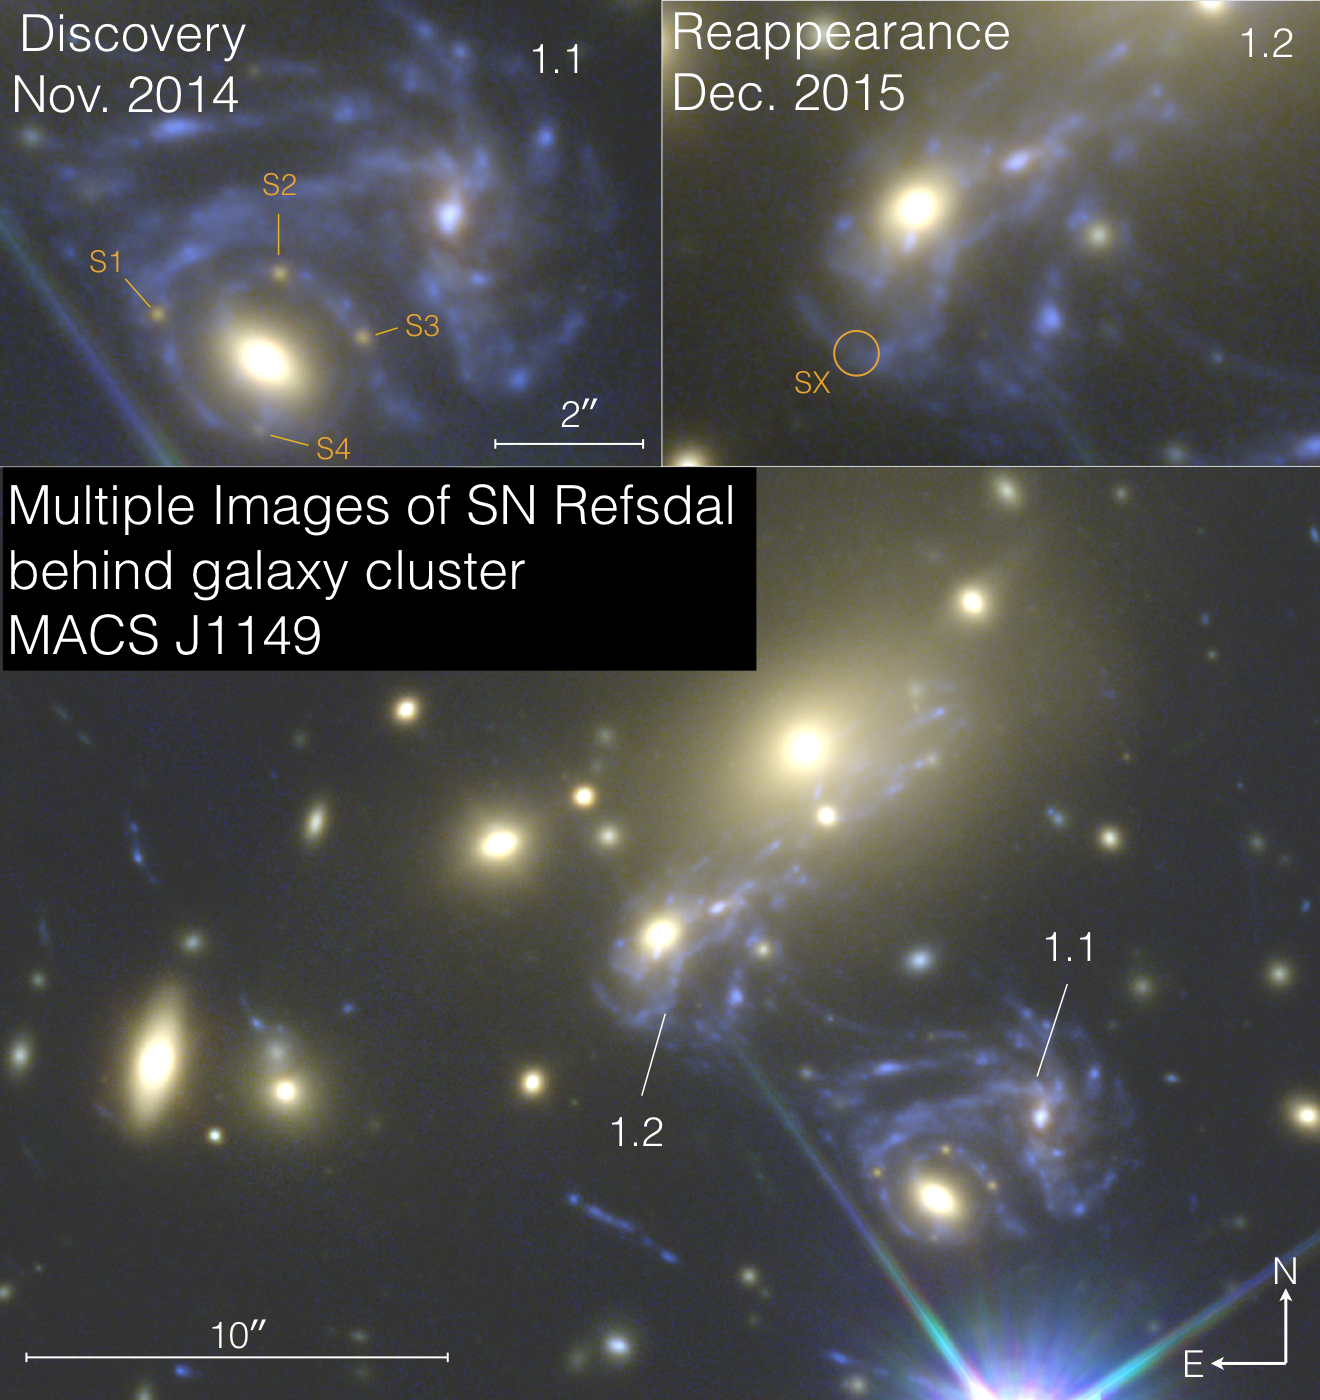
\includegraphics[width=.5\linewidth]{FIG/refsdal_summary}
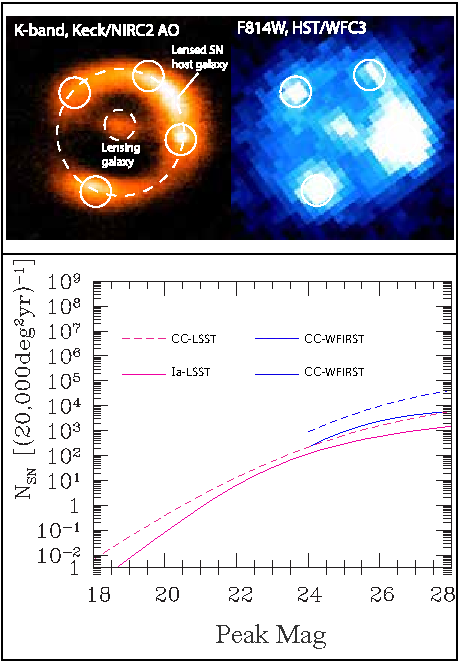
\includegraphics[width=.37\linewidth]{FIG/lensed3}
\caption{
(Left) MACS J1149.6+2223 field, showing the positions of the three primary
images of the SN Refsdal host galaxy. SN
Refsdal appears as four point sources in an Einstein Cross
configuration in the southeast spiral arm of image 1.1 \citep{Rodney:2016}. (Right)
Expected numbers of SN Ia and Core Collapse}
\end{figure}%

As a previously ignored check against systematic biases, our reanalysis will use both the \textit{PythonPhot} and the \textit{DOLPHOT} packages to 
perform photometric measurements. We will also measure the photometry in single-exposure images, allowing us to check for any deviations 
at very short timescales, indicative of very rapid microlensing events. \cite{Rodney:2016} measured flux using a single empirical 
point-spread function (PSF) fixed in time, derived from standard stars. However, as we know that the HST PSF does undergo 
subtle variations due to telescope ``breathing" \citep{Dressel:2012}, our re-analysis will use foreground stars within the MACS1149 imaging 
datasets to define a variable PSF model \citep{Cox:2011}. \textbf{The reduction of systematic biases in the photometry and our improvements to the 
PSF will provide drastically ameliorated flux calculations, which in turn will increase the accuracy and precision of time delay measurements.}

Microlensing refers to small-scale gravitational lensing
perturbations due to massive objects along the light path of any one image of a
multiply-imaged SN. The effect of microlensing is to cause distortions in the SN light
curves that significantly limit the precision that can be achieved in the measurement of 
their time delays \citep{Dobler:2006}. Despite noting this significant source of uncertainty, the analyses performed for SN Refsdal and SN iPTF16geu 
have completely ignored microlensing due to its complexity (\cite{More:2016,Rodney:2016}). In preparing this proposal, we have already 
used flexible functions to preliminarily measure the effects of the type 1 microlensing on SN Refsdal (Figure 2), and it's 
\textbf{clear that microlensing must be taken into account} in order to ensure accurate time delay and magnification measurements. 
Therefore, we will \textbf{fully analyze the effects of microlensing on a multiply-imaged SN for the first time} and ensure they can be accurately
accounted for in future SN analysis.

\textbf{The next decade is expected to yield observations
of over 100 lensed SNe} that will require analysis \citep{Oguri:2010},
yet \textbf{there is no public software package for analyzing multiply-imaged SNe.}
In the course of this work, we are producing an open-source software package written 
in Python for use in this and future SN analysis. Specifically, efforts to measure the time 
delays of SN iPTF16geu, critical to a new measurement of $H_0$, have not been 
successful beyond broad constraints (\cite{Goobar:2016}, \cite{More:2016}). This new tool,
developed and tested in the course of reanalyzing SN Refsdal, will be used to make a time 
delay measurement in parallel to the Goobar et al. team when they make follow-up observations
later this year, providing an important independent check of such a measurement for the first time. 

The discovery of SN iPTF16geu suggests that the \textbf{rate of strongly lensed Type Ia SNe is likely much higher than
previously thought}, with implications for our constraints on $H_0$, the study of galaxy sub-structures,
and tests of theories of modified gravity (\citet{Goobar:2016},\citet{More:2016}). If the number of lensed Type Ia SNe observed in the LSST/WFIRST
era follows these predictions, then it will be absolutely essential to have a publicly available, standardized 
tool in place to accurately produce time delay and magnification measurements. The reanalysis of SN 
Refsdal offers a \textbf{unique chance} to develop the software and methodology necessary in the coming years for
analyzing new SNe \textbf{to obtain exciting scientific results}, including constraints on dark energy parameters and a
direct probe of the expansion rate of the universe, $H_0$.

\begin{figure}[h]
\centering
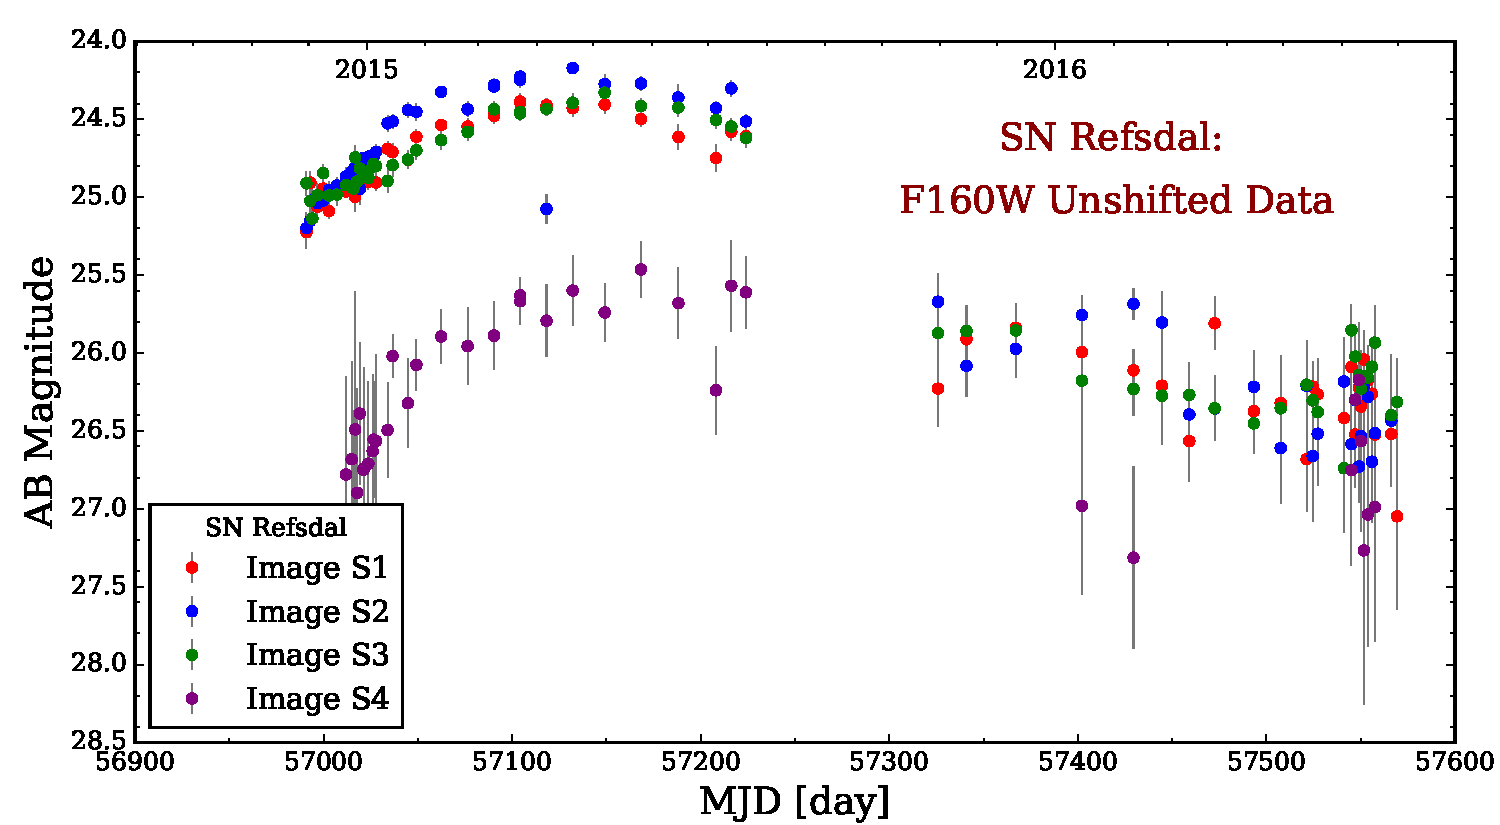
\includegraphics[width=.7\textwidth]{FIG/points_plot_2017.pdf}
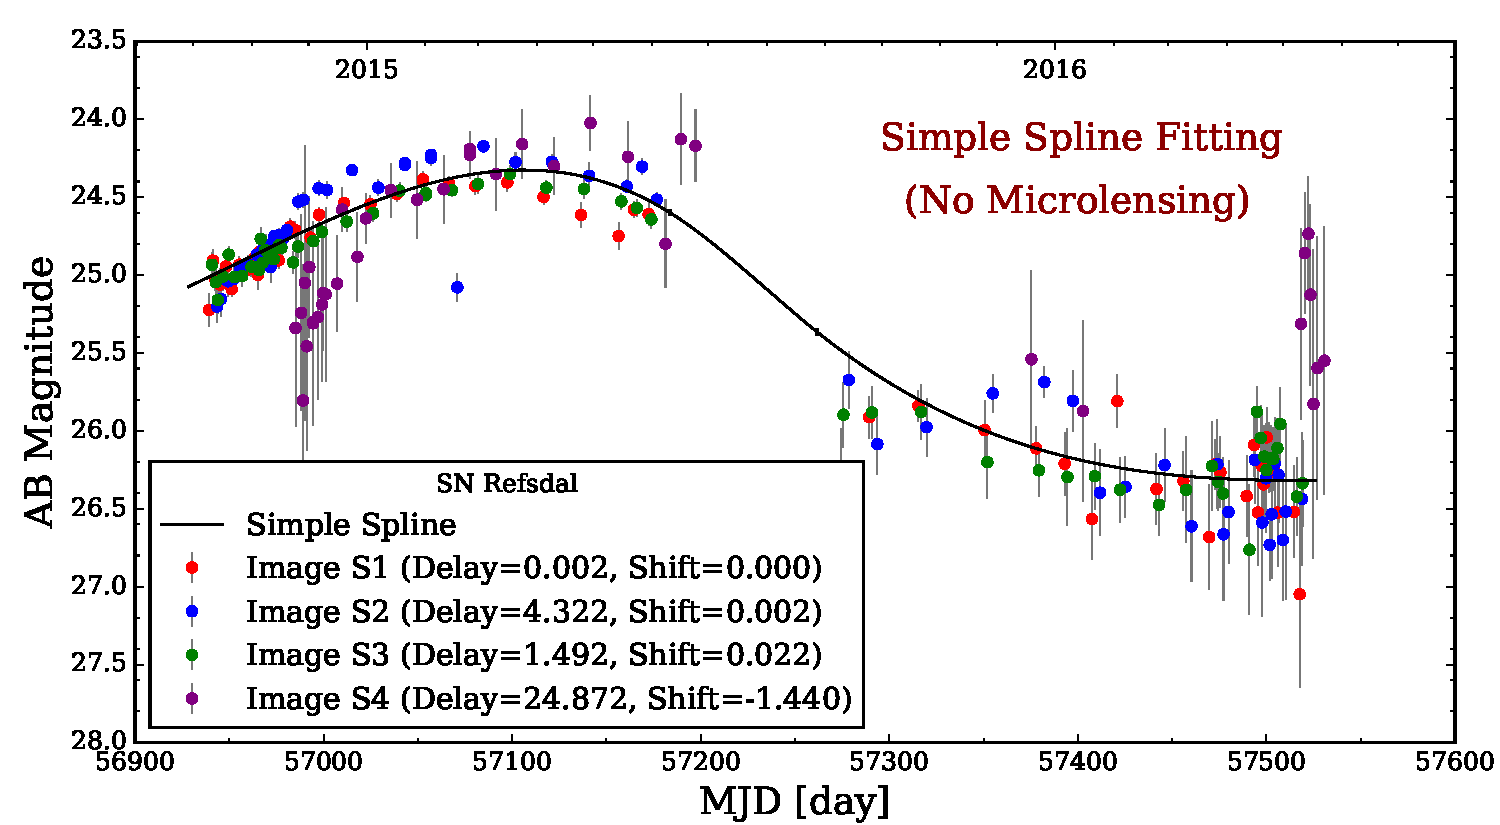
\includegraphics[width=.7\textwidth]{FIG/refs_plot_2017.pdf}
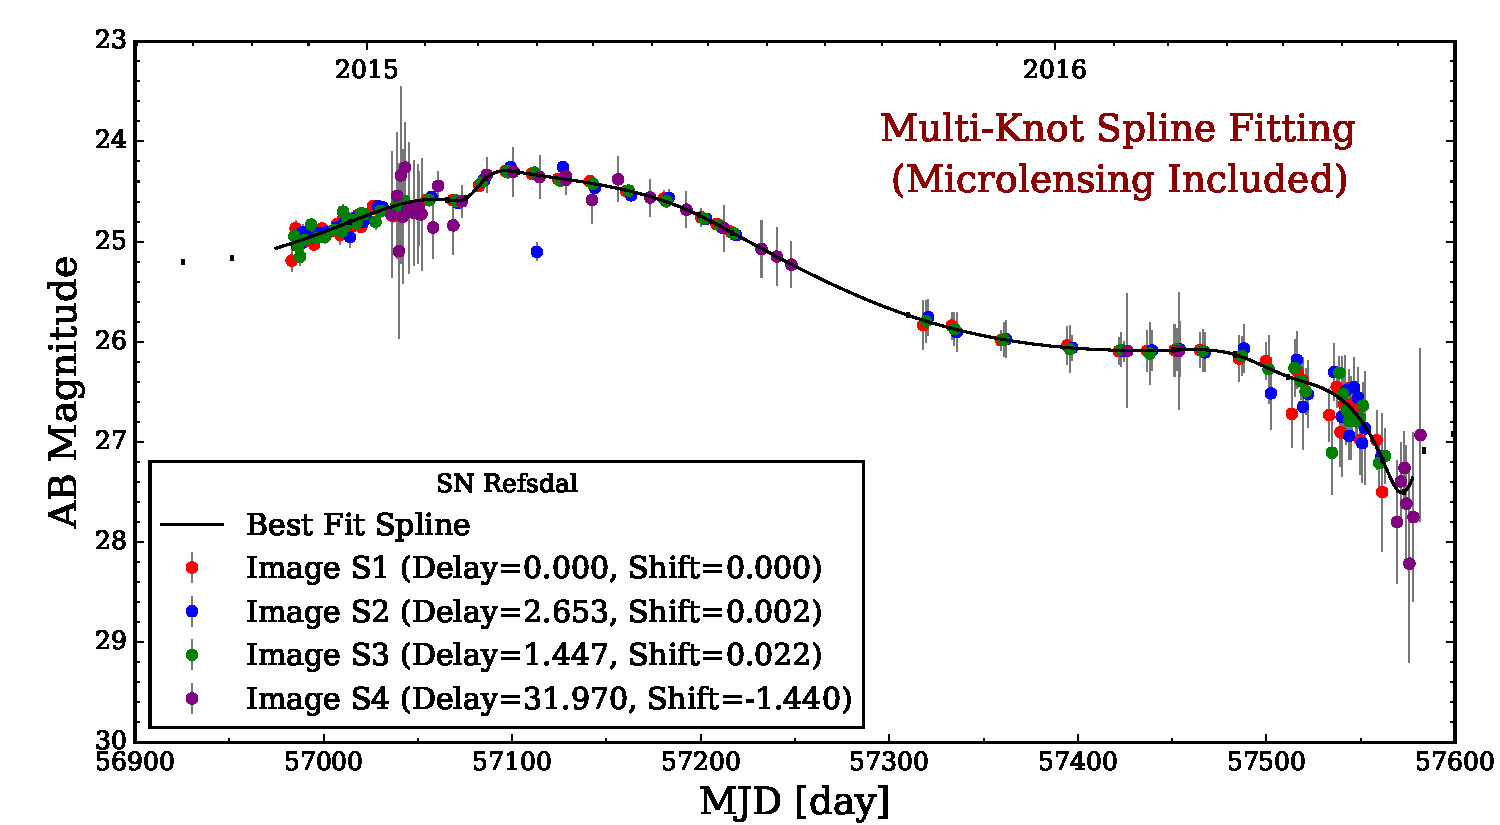
\includegraphics[width=.7\textwidth]{FIG/spline_plot_2017.pdf}
\caption{(Top) HST F160W data representing the four images of SN
Refsdal (Figure 1), with no lensing or time shifts. (Middle) Method of
fitting the SN Refsdal light curves from Rodney et al. 2016, which did
not consider microlensing effects. (Bottom) Preliminary results from 
this work using a multi-knot spline to fit the data. This method 
includes microlensing effects, which leads to a slight adjustment in 
time delay measurements. }
\end{figure}

\bigskip
 
 




